\documentclass[a4paper, 11pt]{exam}
\usepackage{titling}
\newcommand{\subtitle}[1]{%
  \posttitle{%
    \par\end{center}
    \begin{center}\large#1\end{center}
    }%
}

\usepackage{url}
\usepackage{amsmath,amsthm,enumitem,amssymb}
\usepackage{algorithm,algorithmic,amsmath}
\usepackage{graphicx}
\usepackage{hyperref}
\renewcommand{\labelenumii}{\roman{enumii}}
\usepackage{courier}
\usepackage{epsfig}

\title{Homework Assignment 4}
\subtitle{CS/ECE 6810: Computer Architecture \\
Nov 28, 2018\\
Jake Pitkin, u0891770}

\author{ \\
\textbf{Memory Systems}}
\date{Due Date: December 11, 2018.\\
(120 points)}

\begin{document}
\maketitle

\begin{enumerate}

\item \textbf {Virtually Indexed Cache.}
Referring to the lecture slide on virtual address translation and TLB, explain the
challenges if the number of bits in the page offset does not equal the number of
bits in the sum of ``Index'' and ``Byte'' (Please see \url{http://www.cs.utah.edu/~bojnordi/classes/6810/f18/slides/18-tlb.pdf}). 
You are asked to identify the issues and their corresponding solutions from the literature.
\textbf{(20 points)}

Let x be the number of page offset bits and y be the number of bits in the sum of "Index" and "Byte". We will consider 3 cases: \\

\textbf{Case x = y:} In this case they are equal, there is no challenge and we can index into the cache in parallel with page number translation by the TLB. This is a side effect of the page offset bits being identical in both the virtual and physical addresses so waiting for the TLB to execute won't change the bits used for "Index" and "Byte". \\

\textbf{Case x $>$ y:} Here we have more page offset bits than required for "Index" and "Byte". We can just use a subset of the page offset bits for "Index" and "Byte" and this is fine for the same reasons as in case 1. \\

\textbf{Case x $<$ y:} When there are less page offset bits than required for "Index" and "Byte" an issue arises. As discussed in the lecture, in this case part of the "Index" bits will come from the virtual address. This means the index into cache will be dependent on the virtual address. Two different virtual addresses could be mapped to a single physical address. As such, it's possible for a given physical word to be put into the cache in more than one location. \\

From the wikipedia on CPU caches, this is called aliasing. This is an issue as we now have cache coherence problems inside a single cache. Processors are designed to satisfy cache coherence under the assumption a given cache only contains a physical word once. There is also the issue of contiguous pages in virtual memory not always being contiguous in physical memory. Using the virtual address for caching could lead to poor performance as we overwrite contiguous pages in physical memory.\\

To solve this issue we must guarantee any given physical word doesn't exist in a cache in more than one location. But we still want to use the virtual address for some of the "Index" bits as it allows us to run the two streams of execution as described in the lecture. As hinted in lecture the solution is cache coloring.\\

From the wikipedia on cache coloring, it is the process of attempting to allocate free pages that are contiguous from the CPU cache's point of view. That is, normally a physically index CPU aims to place contiguous pages in physical memory in different positions in the cache. But with page coloring: \textit{Physical memory pages are "colored" so that pages with different "colors" have different positions in CPU cache memory. When allocating sequential pages in virtual memory for processes, the kernel collects pages with different "colors" and maps them to the virtual memory. In this way, sequential pages in virtual memory do not contend for the same cache line} (from the wikipedia on cache coloring). \\

This solves our performance problem as sequential pages in virtual memory do not content for the same cache line. When using some of the virtual address bits for "Index" we use the lower bits. As such, contiguous pages in virtual memory will be assigned different positions in the cache. Additionally this solves the problem of aliasing. If two virtual addresses map to the same physical address, they will be assigned to the same line in the cache (as the physical address with have a given color) and we won't have duplicate entries and cache coherence problems.

\textbf{References:}

Lecture 18 video: https://web.microsoftstream.com/ \\ video/8d07bb10-4791-4c46-bab8-1b2e2a7e1a09 \\

Lecture 18 slides: http://www.cs.utah.edu/~bojnordi/classes/6810/f18/slides/18-tlb.pdf \\

Wikipedia on caches: https://en.wikipedia.org/wiki/CPU\_cache \\

Wikipedia on cache coloring: https://en.wikipedia.org/wiki/Cache\_coloring

\item \textbf {Virtual Memory and TLB.}
Consider an operating system (OS) using 1KB pages for mapping virtual to physical addresses.
Initially, the TLB is empty and all of the required pages for the user application as well as the page table are stored in the main memory.
(There is no need to transfer data between main memory and the storage unit.)
Every access to the TLB and main memory takes respectively 1 and 200 processor cycles.
The TLB can store up 16 entries.

\begin{enumerate}
	\item Assuming that the main memory size is 1MB and the page table has 2048 entries, show the number of required bits for the physical and virtual address fields. \textbf{(5 points)}
	
	1KB pages = $2^{10}$ = 10 offset bits to index \\
	2048 page table entries = $2^{11}$ =  11 bits to address \\
	1MB main memory with 1KB pages = $2^{20} / 2^{10}$ = 10 bits to address
	
	\fbox{\parbox{\linewidth}{
	Virtual address = Virtual Page No + offset = 11 + 10 = 21 bits \\
	Physical address = Page frame No + offset = 10 + 10 = 20 bits}}
	\item Assume that the user application only generates five memory requests to the virtual addresses \texttt{0000}, \texttt{0004}, \texttt{0008}, \texttt{0800}, and \texttt{0804} (all in hexadecimal);
	the first request is ready at time 0; and
	the processor generates every next request immediately after serving the current one.
	Please find the execution time with and without using TLB in the proposed system and compute the attainable speedup due to using TLB.
	\textbf{(15 points)}
	
	\fbox{\parbox{\linewidth}{Answer}}
\end{enumerate}






\item \textbf {DRAM Address Mapping.}
Consider a simple in-order DRAM command scheduler.
Initially, all DRAM banks are precharged and the scheduling queue contains seven read requests to the following physical addresses: 
\texttt{00040108},
\texttt{01040101},
\texttt{FF042864},
\texttt{A5181234},
\texttt{A5184321},
\texttt{00161804}, and
\texttt{01040104}
(all in hexadecimal).
Using the following address mapping scheme, show all the required commands issued by the controller to serve the memory requests.
\textbf{(20 points)}

\begin{center}
	\begin{tabular}{|c|c|c|c|c|}
		\hline
		row (10)&bank (4)&rank (2)&channel (0)&column (16) \\
		\hline
	\end{tabular}
\end{center}

\fbox{\parbox{\linewidth}{\begin{center}
	\begin{tabular}{ |c|c| } 
		\hline
		\textbf{Physical Address}& \textbf{Commands}\\ 
		\hline
		\texttt{00040108} & \\ \hline
		\texttt{01040101} & \\ \hline
		\texttt{FF042864} & \\ \hline
		\texttt{A5181234} & \\ \hline
		\texttt{A5184321} & \\ \hline
		\texttt{00161804} & \\ \hline
		\texttt{01040104} & \\ \hline
	\end{tabular}
\end{center}}}

\item \textbf{DRAM Row (Page) Management.}
A computer system includes DRAM and CPU.
The DRAM subsystem comprises a single channel/rank/bank.
CPU generates a sequence of memory requests to rows \texttt{X} and \texttt{Y}.
Table below shows the accessed rows by the memory requests and their arrival times at the DRAM controller.
Assume that the DRAM bank is precharged initially; the DRAM scheduling queue has infinite size; and the memory interface must enforce the following timing constraints (all in $ns$):
tCAS = 3, tRAS = 20, tRP = 20, tRCD = 10, and tBURST = 4. 

\begin{center}
	\begin{tabular}{|c|c|}
		\hline
		\textbf{Accessed Row} & \textbf{Arrival time ($ns$)} \\
		\hline
		\texttt{X}  & 10 \\
		\hline
		\texttt{X}  & 70 \\
		\hline
		\texttt{Y}  & 80 \\
		\hline
		\texttt{X}  & 85 \\
		\hline
		\texttt{Y}  & 110 \\
		\hline
		\texttt{X} & 210 \\
		\hline
	\end{tabular}
\end{center}

The goal is to evaluate two row management policies, namely \textit{open-page} and \textit{closed-page}.
Show all the necessary transactions on the command, address, and data buses for each policies.
Discuss which policy performs better for the given example.
(Note: you are allowed to reorder requests already waiting in the memory controller.)
\textbf{(20 points)}
\begin{figure}[h!]
	\begin{center}
		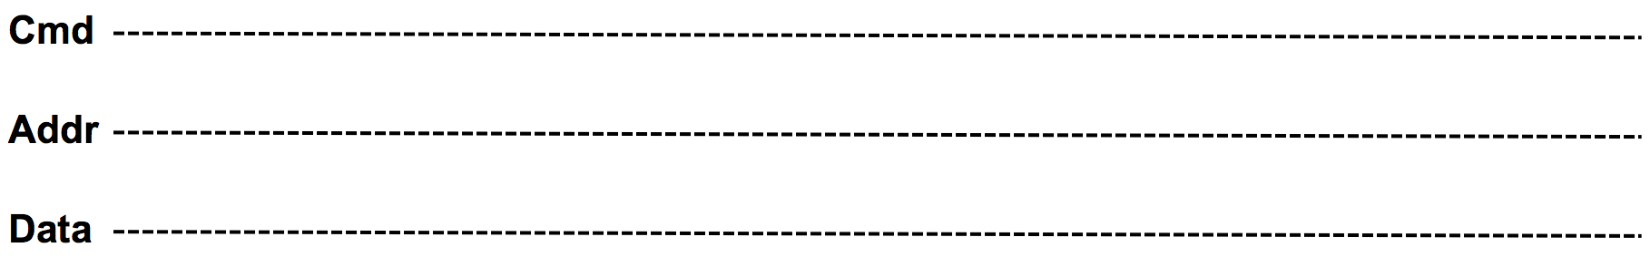
\epsfig{file=timing.pdf, width = \columnwidth}
	\end{center}
\end{figure}

\fbox{\parbox{\linewidth}{Answer}}

\item \textbf{Data TLB.}
Consider the following  pseudo code, in which \textbf{X} and \textbf{Y} are allocated as contiguous integer arrays in memory and are aligned to the 4KB boundaries.
Assume that \textbf{k} and \textbf{l} are allocated in the register file with no need for memory accesses.
We execute the code on a machine with virtual memory where the integer type (\textbf{int}) is 4 bytes wide.
Assume that the system include a direct-mapped D-TLB with 1024 entries for serving all data accesses only.
Initially, the D-TLB is empty.
Find the hit rate of the D-TLB when running the code.
\textbf{(20 points)}
\begin{algorithm}
	\textbf{\#define M 1024} \\
	\textbf{int X[M*M];} \\
	\textbf{int Y[M*M];} \\
	\textbf{int k, l;}
	\begin{algorithmic}	
		\FOR{$(k = 0; k < M; k++)$}
		\FOR{$(l = 0; l < M; l++)$}
		\STATE \texttt{Y[l*M+k] = X[k*M+l];}
		\ENDFOR
		\ENDFOR
	\end{algorithmic}
\end{algorithm}

\fbox{\parbox{\linewidth}{Answer}}

\end{enumerate}
\end{document}
